\chapter{Secure Access Module}
\label{chapter3}

\section{Introduzione}
Le Smart Card sono un esempio di token crittografico, ovvero di un dispositivo hardware utilizzato per effettuare un'autenticazione (di solito a due fattori).

Il funzionamento del token è quello di generare codici numerici pseudocasuali periodicamente basandosi su algoritmi che prendono in considerazione il tempo dato da un orologio interno al dispositivo e dati come il codice di serie. Lo stesso algoritmo viene fatto girare su un server che è stato sincronizzato col token e che quindi produce gli stessi codici.

I numeri generati, insieme a un codice PIN fornito all'utente generano una password temporanea di sessione, valida cioè per un periodo limitato. L'autenticazione viene detta a due fattori perchè richiede sia la conoscenza del PIN che il possesso del token (univoco).

Il token rende un accesso molto più sicuro in quanto la password generata è valida per un periodo di tempo limitato, quindi un eventuale malintenzionato che volesse tentare di indovinare la password ha un tempo molto limitato per trovarla ed utilizzarla.
\cite{wiki_token}

Sebbene le smart card sono tra i token crittografici più diffusi al giorno dopo, le stesse funzionalità sono implementate da circuiti integrati saldati sulle schede di dispositivi più ampi dai quali sono utilizzati. Questi circuiti sono noti come dispositivi SAM (\textit{Secure Access Module}) e possono essere trovati in apparecchiature come i POS o i bancomat.

I SAM spesso vengono utilizzati come posti sicuri per conservare chiavi di crittografia in modo tale che non debbano più uscire dal dispositivo, impedendo che utenti malintenzionati possano accedervi. Tuttavia possono anche essere utilizzati come proxy per ottenere una comunicazione più sicura con una smart card.

Quando un'applicazione deve accedere alla smart card per comunicare può utilizzare il SAM come tramite per fare in modo che i dati che vengono scambiati con la card siano criptati come mostrato in figura \ref{fig:proxy_sam}.

\begin{figure}[h!]
  \centering
  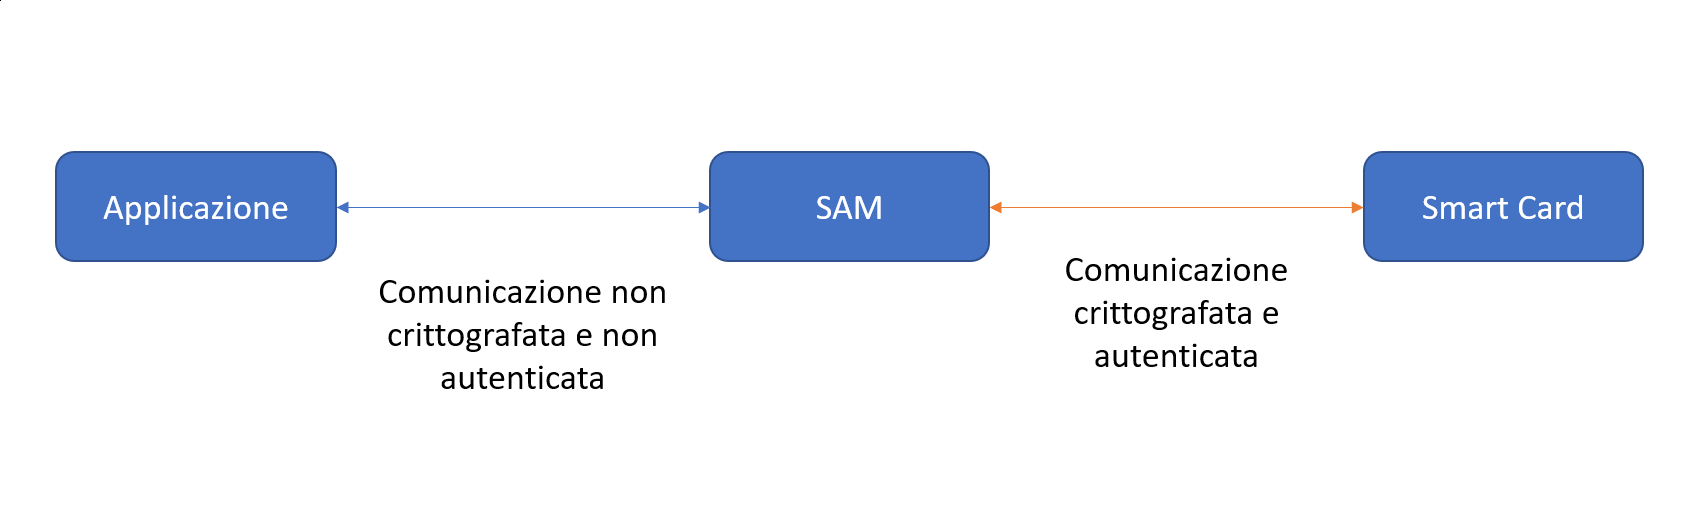
\includegraphics[width=410pt]{pictures/proxy_sam.png}
  \caption{Schema della comunicazione utilizzando un SAM.}
  \label{fig:proxy_sam}
\end{figure}

In alternativa le SAM posso essere utilizzate per generare o calcolare chiavi di sessione o crittografare piccoli hash, similmente a una smart card, che può essere considerata un tipo particolare di SAM.

\section{Point of sale}
Il POS (\textit{Point of sale}) è un dispositivo elettronico utilizzato dai commercianti per dare la possibilità ai loro clienti di acquistare merci e/o servizi tramite l'utilizzo di moneta virtuale (carte di credito o bancomat).

Il funzionamento di un POS è molto semplice, prima di tutto il terminale deve leggere la carta del cliente e verificarne la validità. Per la lettura vi sono varie tecnologie disponibili, dalla ormai inutilizzata banda magnetica, alla lettura della smart card a contatti presente sulla carta, alla più recente tecnologia contactless che prevede l'avvicinamento della carta al dispositivo senza effettivamente toccarlo. Quest'ultima opzione può essere anche sfruttata per pagare con il cellulare tramite i servizi offerti da Google e Apple.

Una volta letta la carta, va autorizzata la transazione. Per farlo vi sono due possibili modi:
\begin{itemize}
    \item Tramite firma. Il POS stampa due scontrini, uno dei quali va lasciato al cliente come ricevuta, mentre l'altro va firmato dallo stesso. Se la firma presente sullo scontrino non è la stessa presente sulla carta, allora la transazione viene considerata fraudolenta.
    \item Tramite PIN. Il cliente inserisce un PIN segreto associato alla carta. Ciò aumenta di molto la sicurezza della transazione.
\end{itemize}

\cite{pos}

\section{Trusted Platform Module}
\label{trusted_platform_module}
Un Trusted Platform Module (o TPM) è un microchip elettronico utilizzato per la sicurezza informatica e implementato nelle schede madri o in altri dispositivi elettronici, può essere considerato un SAM in senso lato. Questi chip sono dotati di una coppia di chiavi e un modulo che implementa la crittografia asimmetrica (RSA) dei dati. Essendo le chiavi diverse per ogni dispositivo, esse permettono di identificarlo univocamente.

\subsection{Specifiche del TPM}
Le specifiche di questo tipo di dispositivi sono state pubblicate dal \textit{Trusted Computing Group}. Le funzionalità che questo dispositivo deve poter offrire sono:
\begin{itemize}
    \item La generazione di numero pseudo-casuali.
    \item La generazione e memorizzazione di chiavi crittografiche asimmetriche.
    \item La cifratura e de-cifratura di dati mediante l'algoritmo RSA.
    \item La generazione e verifica di hash SHA1
\end{itemize}
Per realizzare queste funzionalità il chip deve avere una serie di componenti che comunicano utilizzando un bus interno e in grado di comunicare con il bus della scheda madre sulla quale il dispositivo è installato.

\subsubsection{Dispositivo I/O}
Come accennato il dispositivo I/O deve essere in grado di far passare le informazioni dal bus interno del chip a quello esterno e viceversa.

\subsubsection{Coprocessore Crittografico}
Il coprocessore crittografico deve essere in grado di garantire le funzionalità che sono state elencate in precedenza. Questo dispositivo può anche utilizzare la crittografia asimmetrica per scambiare dati internamente. Inoltre per la firma digitale si usano chiavi a 2048 byte anche se il modulo deve comunque supportare chiavi a 512 e 1024 byte.

\subsubsection{Generatore di Chiavi Crittografiche}
Questo dispositivo deve semplicemente generare una coppia di chiavi crittografiche secondo L'Algoritmo RSA. Non ci sono specifiche sul tempo necessario per il calcolo, che può essere arbitrariamente lungo.

\subsubsection{Motore HMAC}
Si tratta di un dispositivo preposto alla verifica che i dati di identificazione siano corretti e al tempo stesso non siano stati manipolati. Per ottenere ciò si utilizza l'algoritmo HMAC con chiavi di 20 byte e blocchi di dati di 64 byte. Questo algorimo, utilizzando una parte del messaggio originale e della chiave per la crittografia dei dati, garantisce massima sicurezza.

\subsubsection{Generatore di Numeri Pseudocasuali}
Il generatore di numeri pseudocasuali serve per introdurre della casualità all'interno del TPM. Viene utilizzato per generare le chiavi asimmetriche per la firma digitale. Questo dispositivo deve essere composto da un componente in grado di ricevere dati imprevedibili e un coprocessore in grado di generare i numeri utilizzando una funzione non invertibile. Ogni volta che viene attivato, il generatore deve fornire 32 byte di dati casuali.

Quando viene prodotto il TPM il generatore viene inizializzato con dati casuali tramite disturbi termici o via software. Una volta inizializzato nessuno (nemmeno il produttore) deve poter essere in grado di modificare lo stato del componente. Durante il suo funzionamento il generatore utilizzerà altri dati imprevedibili come ad esempio il movimento del mouse o i tasti premuti sulla tastiera. Infine la funzione di output riceve un numero minore di input per produrre i dati necessari, in modo da creare ambiguità e garantire l'invertibilità della funzione utilizzata.

\subsubsection{Motore SHA-1}
Tale componente viene utilizzato per la firma digitale dei file e deve poter gestire hash SHA-1 da 160 bit.

\subsubsection{Gestore di alimentazione}
Questo dispositivo non solo deve alimentare il TPM, ma deve anche informare i suoi dispositivi interni dello stato dell'alimentazione. Ciò per evitare che possano essere collegati altri dispositivi (operatori esterni) non autorizzati al chip.

\subsubsection{Opt-In}
Questo componente ha il compito di gestire l'accensione, spegnimento, attivazione e disattivazione del TPM non ché la presenza di operatori esterni collegati al dispositivo. L'Opt-In deve garantire che le operazioni di accensione/spegnimento e attivazione/disattivazione del TPM sono effettuate da utenti abilitati al controllo del TPM (\textit{TPM-Owner}).

\subsubsection{Motore di esecuzione}
Il compito del motore di esecuzione è quello di eseguire il codice che il chip riceve dal dispositivo di Input/Output garantendo la trasparenza delle operazioni eseguite e la protezione dei dati sensibili.

\subsubsection{Memoria non volatile}
L'ultimo componente che troviamo nel TPM è una memoria non volatile utilizzata per memorizzare i dati che identificano il TPM. Questa memoria deve poter essere letta solo dal proprietario del modulo per poter conservare i dati in maniera sicura.

\subsection{Utilizzo del TPM}
Il TPM, per essere utilizzato, richiede un software particolare, ovvero uno specifico \textit{Trusted Software Stack}, definito anch'esso dal Trusted Computing Group.

Utilizzando il software giusto il TPM è in grado di attestare da remoto l'identità della macchina su cui è montato e di cifrare e decifrare i dati che viaggiano da e verso la memoria di massa (quest'ultimo processo è denominato \textit{data sealing} e \textit{data binding}).

Il processo di data sealing consiste nella cifratura dei dati che vengono salvati sulla memoria di massa del PC tramite l'utilizzo di una chiave che dipende dallo stato del computer (ovvero dall'hardware e il software utilizzato in quel momento). Ne consegue che la de-cifratura dei dati può essere fatta solo calcolando la medesima chiave e quindi avendo un PC il cui hardware e software in esecuzione corrisponda a ciò che è stato utilizzato per cifrare i dati.

Il binding dei dati, invece, consiste nella cifratura delle informazioni usando una chiave RSA detta \textit{Endorsment Key} che identifica univocamente il TMP, garantendo, quindi, che i dati possono essere decifrati solamente dal chip utilizzato per cifrarli.

L'attestazione della macchina viene fatta con apposite chiavi dette \textit{Attestation Identity Key} (AIK) generate dal TPM. Tuttavia dalla versione 1.2 è possibile anche utilizzare un protocollo che preserva la riservatezza dei dati del sistema operativo, denominato \textit{Direct Anonymous Attestation}. In sostanta il chip ha particolari registri detti \textit{Platform Configuration Register} (PCR) che utilizza per salvare un hash dell'evoluzione dello stato del sistema effettuando un controllo sull'hardware e software installato e misurandolo secondo la formula \ref{Eq:pcr}.
    \begin{equation}
   	PCR[i]_{t1} = SHA1(PCR[i]_{t0} + informazioni\_prelevate_{t1})
    	\label{Eq:pcr}
    \end{equation}
    
In altre parole, il contenuto dell'i-esimo registro viene aggiornato (al tempo \textit{t1}) con l'hash del contenuto presente nel registro al tempo precedente (ovvero \textit{t0)} più le informazioni prelevate al tempo \textit{t1}. Quando il sistema è evviato il contenuto del PCR è azzerato.

Disponendo delle informazioni conenute nel PCR, il software può autenticare la macchina e decidere quali operazioni intraprendere.
\cite{wiki_tpm}